% !TeX root = main.tex
\chapterimage{chapter-02-concetti-fondamentali.jpg}
\chapter{Concetti fondamentali di informatica}\label{fondamentali-di-informatica}

In questo capitolo introduciamo alcuni concetti chiave dell'informatica. Per far sì che i tuoi alunni e alunne inizino a sviluppare la capacità di approcciare il mondo e risolvere i problemi anche con una lente computazionale, è importante conoscere questi ``ingredienti'' di base: idee semplici ma molto potenti alla base di ogni programma o sistema informatico. Alcuni termini ti suoneranno familiari, ma in informatica assumono un significato specifico che è importante chiarire.

\section{Informatica: la scienza dell'elaborazione automatica }\label{informatica-la-scienza-dellelaborazione-automatica}

Così come l'oggetto di studio principale dell'astronomia non sono i telescopi, ma gli astri e l'universo, e così come l'oggetto di studio principale della biologia sono gli esseri viventi, e non i microscopi, così l'oggetto principale di studio dell'informatica \textbf{non} sono i computer. Al contrario, l'informatica studia l'\textbf{elaborazione automatica dell'informazione}: nelle prossime sezioni proviamo a capire, per ciascun concetto, che cosa significa.

\section{Informazioni e dati }\label{informazioni-e-dati}

\textbf{L'informazione è una conoscenza utile} per le persone, rispetto ad un determinato obiettivo. Ad esempio, può essere utile conoscere l'età di un bambino perché alcune attività sportive della scuola sono riservate ai bambini ``dai 10 anni in su''.

Per \textbf{esprimere questa stessa informazione, possiamo usare dati diversi} \parencite{lonati-monga-2025}: l'anno di nascita del bambino, la sua data di nascita completa, oppure il numero di anni compiuti. Alcuni dati sono più precisi di altri: soprattutto se l'attività è all'inizio dell'anno, può fare la differenza sapere anche il giorno e il mese di nascita per capire se, a quella data, il bambino avrà già compiuto 10 anni oppure no. I dati, da soli, non hanno significato (per esempio: ``10'', ``2015'', ``07/03/2015''). Diventano significativi solo all'interno di una convenzione e di un contesto d'uso: se decidiamo che ``07/03/2015'' rappresenta la data di nascita di una persona, allora possiamo interpretare quel dato come utile per esprimere una certa informazione (ad esempio per stabilirne l'età).

Sebbene quindi sia più preciso dire che l'informatica si occupa dell'elaborazione automatica delle rappresentazioni dei dati che esprimono una certa informazione, per brevità nel seguito parleremo di elaborazione dei dati o di elaborazione dell'informazione.

\subsection{Elaboratori }\label{elaboratori}

Ora immaginiamo di avere l'elenco di tutte le date di nascita degli alunni e delle alunne della scuola, con centinaia o migliaia di nomi, e di voler calcolare, per ciascuno, l'età precisa in un certo giorno. Farlo a mano richiederebbe moltissimo tempo. È qui che l'Informatica ci viene in aiuto: ci consente di \textbf{elaborare automaticamente questi dati}.

Oggi abbiamo a disposizione dei ``macchinari'' (potrebbe capitare di sentire gli informatici chiamarli ``macchine'': non stanno parlando di automobili!): i \textbf{computer}\footnote{Molti traducono \emph{computer} con \emph{calcolatore}, ma qui sceglieremo invece \emph{\textbf{elaboratore}}, per porre maggiore attenzione sul loro scopo principale, che è appunto l'elaborazione automatica dei dati.}.

Il ``macchinario computer'' avrà al suo interno meccanismi specifici\footnote{Solitamente con il termine \textbf{architettura} si indicano le parti principali di un computer (ad esempio processore, memoria e dispositivi di input/output) e come ``collaborano'' tra loro per farlo funzionare.} (pensiamoli, per il momento, come interruttori e ingranaggi). La disposizione interna degli interruttori (acceso/ spento) in un dato momento, detta \textbf{stato}, può rappresentare determinati dati. Gli ingranaggi, opportunamente progettati, potranno compiere fisicamente l'elaborazione (accendere/ spegnere alcuni interruttori) e quindi portare la macchina a uno stato diverso, che sarà il risultato dell'elaborazione.

Un computer moderno potrebbe avere decine o centinaia di miliardi di interruttori (che, in questo contesto, si chiamano \textbf{transistor} e sono componenti elettronici).

\subsection{Rappresentare numeri con ``interruttori'' }\label{rappresentare-numeri-con-interruttori}

La prima sfida è quindi rappresentare qualsiasi informazione (o, più precisamente, qualsiasi dato che usiamo per esprimerla) esclusivamente mediante interruttori.

Dobbiamo quindi riuscire a rappresentare numeri, lettere, colori, immagini e suoni utilizzando solo interruttori.

Per i numeri è relativamente semplice. Il nostro sistema numerico è posizionale, cioè il valore di ciascuna cifra è stabilito dalla sua posizione, ed è decimale, cioè in base \(10\). Per esempio, il numero \(2025\), in base \(10\), ha, leggendolo da destra a sinistra, la cifra \(5\) nella posizione delle unità, \(2\) in quella delle decine, \(0\) in quella delle centinaia e \(2\) in quella delle migliaia. In notazione polinomiale: $2025 = 2 \cdot 10^{3} + 0 \cdot 10^{2} + 2 \cdot 10^{1} + 5 \cdot 10^{0}$.


Se invece di usare un sistema in base \(10\) ne usiamo uno in base \(2\), che ha due cifre soltanto (\(0\) e \(1\)), possiamo dire che il numero $2025$ si scrive
$(11111101001)_2$,
cioè
\begin{center}
\setlength{\jot}{6pt}
\(\displaystyle
\begin{gathered}
  (11111101001)_2 = {}\\
  1\cdot2^{10} + 1\cdot2^{9} + 1\cdot2^{8} + 1\cdot2^{7} + 1\cdot2^{6} + 1\cdot2^{5} + 0\cdot2^{4} + 1\cdot2^{3} + 0\cdot2^{2} + 0\cdot2^{1} + 1\cdot2^{0} = {}\\
  1024 + 512 + 256 + 128 + 64 + 32 + 8 + 1 = {}\\
  2025.
\end{gathered}
\)
\end{center}

Possiamo allora rappresentare la cifra \(1\) con un interruttore acceso e la cifra \(0\) con un interruttore spento (ma potremmo anche fare il contrario: l'importante è mettersi d'accordo).

In questo modo possiamo rappresentare tutti i numeri\footnote{Interi non negativi, ma esistono ovviamente altre codifiche, più complesse, per gli altri numeri} che vogliamo (con un numero finito di cifre binarie, in inglese \emph{binary digit}, abbreviato in \textbf{bit}\footnote{Per ragioni storiche e tecnologiche, chiamiamo \textbf{byte} una sequenza di \(8\) \textbf{bit}.}). Ovviamente, più grande è il numero, più bit ci servono.

\subsection{Rappresentare lettere e simboli }\label{rappresentare-lettere-e-simboli}

Per non complicarci la vita, possiamo sempre passare dai numeri, e quindi decidere che ogni \textbf{carattere} (lettera, cifra, simbolo, emoji, ...) viene rappresentato da un numero, e quel numero, abbiamo già visto come rappresentarlo sotto forma di interruttori.

L'associazione carattere-numero è detta \textbf{codice} o \textbf{sistema di codifica}, e, di nuovo, l'importante è mettersi d'accordo. Per esempio, il codice Unicode è uno standard internazionale, e associa ogni carattere a un numero. Ad esempio:

\begin{center}
\begin{tabular}{|p{0.20\linewidth}|p{0.25\linewidth}|p{0.43\linewidth}|}
\hline
\textbf{Carattere} & \textbf{Numero in base 10} & \textbf{Numero in base 2} \\
\hline
! & 33 & 100001 \\
A & 65 & 1000001 \\
a & 97 & 1100001 \\
b & 98 & 1100010 \\
Ω & 937 & 1110101001 \\
爱 & 29233 & 111001000110001 \\
\emoji{smiling-face-with-smiling-eyes} & 128522 & 11111011000001010 \\
\hline
\end{tabular}
\end{center}

\subsection{Rappresentare colori, immagini, video }\label{rappresentare-colori-immagini-video}

Se ti avvicini molto ad uno schermo di un computer (meglio se vecchio), vedrai dei quadratini. Semplificando, dietro a ciascun quadratino che forma il pezzettino dell'immagine che vedi sullo schermo (un ``elemento di un'immagine'', in inglese picture element, cioè \textbf{pixel}) ci sono tre lampadine (led) colorate: una rossa, una verde e una blu. Cambiando l'intensità di ciascuna lampadina, possiamo ottenere una enorme varietà di colori (es. se le accendiamo tutte e tre alla massima intensità avremo tantissima luce: il bianco; se le spegniamo tutte e tre, avremo il nero; se accendiamo totalmente solo quella rossa avremo il rosso; se accendiamo totalmente quella rossa e per metà quella verde, avremo un bell'arancione). Nota che non stiamo lavorando con le tempere su un foglio: qui più colore (più luce) aggiungiamo, più andiamo verso il bianco: ad esempio, tanto verde+tanto blu = azzurro.

L'intensità di Rosso, Verde, Blu (Red, Green, Blue--\textbf{RGB}) può essere espressa, ad esempio (di nuovo, per convenzione e per ragioni tecnologiche), con un numero compreso tra 0 (lampadina spenta) e 255 (lampadina completamente accesa), e dunque ad esempio un bel blu potrebbe essere 51, 102, 255.

Con tanti pixel in griglia si forma un'immagine; con tante immagini mostrate velocemente, una di seguito all'altra, si forma un video.

\section{Elaborare dati }\label{elaborare-dati}

Speriamo di averti convinto, almeno un po', che, tramite milioni di interruttori, è possibile rappresentare tutti i dati che vogliamo. Ma quello che vogliamo fare è anche elaborare questi dati--anzi, farlo fare ai computer!

I computer (oggi tramite circuiti elettronici) possono modificare quali interruttori sono accesi e quali spenti, cioè eseguire \textbf{operazioni sugli interruttori}\footnote{Anche queste operazioni, essendo informazioni/dati, vengono rappresentate all'interno del computer tramite interruttori.}: operatori logici (leggendo l'interruttore acceso come ``Vero'' e spento come ``Falso'', ad esempio accendendo un bit solo se altri due sono già accesi), semplici operazioni aritmetiche sui bit, trasferimento di bit da/verso la memoria del computer, confronti e salti verso un'altra istruzione.

La potenza sta nel fatto che un computer moderno può eseguire \textbf{decine di miliardi di queste operazioni ogni secondo}.

Il computer non ha alcuna idea del significato che noi esseri umani attribuiamo a queste operazioni: si tratta semplicemente di ingranaggi (circuiti elettronici) che accendono o spengono interruttori secondo la logica da noi definita. Il computer, inoltre, non può compiere altre operazioni se non quelle poche e semplici che abbiamo elencato, ma combinandone migliaia in modo sapiente, possiamo compiere elaborazioni molto avanzate.


\section{Competenze digitali o competenze informatiche?}

I computer (inclusi, ad esempio, smartphone, tablet, elettrodomestici smart) vengono quindi chiamati \textbf{dispositivi digitali} proprio perché rappresentano ed elaborano dati rappresentati in modo discreto (tramite cifre binarie, ``binary digit'' o bit).

Ma quando si parla di \textbf{competenze digitali}, si fa riferimento solo alla \emph{``padronanza di uso efficace, sicuro e consapevole di dispositivi, strumenti e tecnologie digitali''} \parencite{mim-indicazioni-2025}. Questo manuale offre invece la possibilità di acquisire \textbf{competenze informatiche}, cioè capire come questi dispositivi possano rappresentare ed elaborare dati in modo automatico, pur seguendo procedimenti ideati dall'uomo.


\section{Istruzioni ed esecutori }\label{istruzioni-ed-esecutori}

Il computer può eseguire solo operazioni molto semplici su dati rappresentati come bit. Per poterlo usare in modo efficace, abbiamo bisogno di descrivere queste operazioni in una forma che sia comprensibile agli esseri umani, ma che possa comunque essere tradotta automaticamente in tali operazioni. Per questo sono stati inventati diversi \textbf{linguaggi formali}, con precise regole sintattiche da rispettare: i \textbf{linguaggi di programmazione}. Essi svolgono proprio questo ruolo: permettono di esprimere in modo chiaro e strutturato le elaborazioni che vogliamo far eseguire al computer, affidando al computer stesso il compito di tradurle nelle corrispondenti operazioni sui bit.

Possiamo quindi ``dimenticarci'' degli ingranaggi e degli interruttori. Dato un linguaggio di programmazione, possiamo supporre che esista un \textbf{esecutore} in grado di ``comprendere'' le istruzioni scritte in quel linguaggio, cioè di eseguirle senza ambiguità. L'esecutore ``non ha dubbi'' su come interpretare l'istruzione: ha modo di eseguirla direttamente o tramite passaggi automatici di traduzione nascosti al programmatore. L'esecutore compirà sempre le stesse operazioni in modo meccanico e totalmente prevedibile in risposta a una stessa istruzione.

Se gli esecutori che abbiamo in mente sono chiaramente i computer, didatticamente può essere utile lavorare con esecutori diversi (ad esempio robot, che sono comunque computer, ma anche esseri umani che ``fanno finta di essere un computer'', come il papà che seguiva passo passo e alla lettera le istruzioni per preparare il panino nel video del Capitolo~\ref{capitolo-1-introduzione}).

Ogni volta che vogliamo far fare qualcosa a un esecutore, dobbiamo esprimerlo tramite un \textbf{linguaggio} per lui ``comprensibile''. In tutte le attività che proponiamo, cerchiamo sempre di chiarire (a meno che il compito non sia proprio quello di inventarle o scoprirle) qual è \textbf{l'insieme di istruzioni che quel particolare esecutore sa eseguire}.

Per descrivere questo insieme, ci serve definire la \textbf{sintassi}, cioè le regole del linguaggio (come si scrivono le istruzioni? Ad esempio: mediante specifiche parole o simboli, indispensabili perché l'esecutore possa ``comprenderle'' ed eseguirle) e la \textbf{semantica}, cioè il significato delle istruzioni in termini di comportamento del programma, un comportamento a cui l'esecutore non assegna un significato come farebbe un essere umano, ma che segue in modo rigoroso e meccanico durante l'esecuzione.

\subsection{Manuale \textit{delle} istruzioni}\label{manuale-delle-istruzioni}

Chiameremo \emph{Manuale delle istruzioni}\footnote{Sappiamo che da un punto di vista grammaticale l'uso di ``delle'' può suonare un po' strano. Tuttavia, il manuale spiega proprio come funzionano le istruzioni (cioè, quali azioni/operazioni l'esecutore compie in risposta a ciascuna istruzione) e non come svolgere l'attività. Per questa ragione, abbiamo scelto l'espressione \emph{Manuale delle istruzioni}.} l'insieme di tutte e sole le istruzioni che un determinato esecutore può eseguire. Per ciascuna istruzione, il manuale indica come esprimerla (es. mediante parole e/o simboli), e quale effetto produce (cioè quali operazioni/azioni l'esecutore compie in risposta a ciascuna istruzione). Non descrive quindi una particolare missione né stabilisce l'ordine delle azioni: definisce il linguaggio con cui sarà possibile costruire tantissimi programmi diversi.

Come esempio, prendiamo Rame, un panda rosso robot che si muove su una griglia quadrata. Rame occupa una casella, ha lo sguardo rivolto verso uno dei quattro lati della casella in cui si trova e sa fare solo tre cose: avanzare di una casella (lungo la direzione in cui è rivolto), ruotare verso sinistra di 90° centrato su se stesso e ruotare verso destra di 90° centrato su se stesso. Non conosce l'obiettivo del programmatore e non interpreta comandi diversi da quelli elencati nel suo manuale: esegue meccanicamente, nell'ordine, le istruzioni che riceve.
\begin{center}
\manualeimpostazioni
\newcommand{\ramefigura}[1]{\vcenter{\hbox{\scalebox{1.8}{#1}}}}
\newcommand{\ramecella}[1]{#1}
\begin{tabular}{|J{\dimexpr0.35\linewidth-2\tabcolsep-4\arrayrulewidth/3\relax}|K{\dimexpr0.15\linewidth-2\tabcolsep-4\arrayrulewidth/3\relax}|K{\dimexpr0.50\linewidth-2\tabcolsep-4\arrayrulewidth/3\relax}|}
\arrayrulecolor{guideManualeBordo}
\hline
\manualetitolo{3}{RAME}
\multicolumn{2}{|c|}{\cellcolor{guideManualeIntestazione}\manualevoceintestazione{ISTRUZIONE}} &
\multicolumn{1}{c|}{\cellcolor{guideManualeIntestazione}\manualevoceintestazione{AZIONE}} \\
\hline
\texttt{VAI AVANTI DI UNA CASELLA} & \ramecella{\scalebox{1.8}{\iconAvanti}} &
\ramecella{\(\ramefigura{\minigrigliarame{1}{2}{0}{0}{0}} \quad\longrightarrow\quad \ramefigura{\minigrigliarame{1}{2}{0}{1}{0}}\)} \\
\hline
\texttt{GIRA A SINISTRA} & \ramecella{\scalebox{1.8}{\iconSx}} &
\ramecella{\(\ramefigura{\minigrigliarame{1}{1}{0}{0}{0}} \quad\longrightarrow\quad \ramefigura{\minigrigliarame{1}{1}{0}{0}{90}}\)} \\
\hline
\texttt{GIRA A DESTRA} & \ramecella{\scalebox{1.8}{\iconDx}} &
\ramecella{\(\ramefigura{\minigrigliarame{1}{1}{0}{0}{0}} \quad\longrightarrow\quad \ramefigura{\minigrigliarame{1}{1}{0}{0}{-90}}\)} \\
\hline
\end{tabular}
\manualeripristinacolore
\end{center}

\medskip

Nelle attività di questa guida non adottiamo fin da subito una definizione rigorosa delle istruzioni, in particolare quando l'esecutore è un essere umano. Questa scelta è intenzionale. Da un lato, il linguaggio naturale è intrinsecamente ambiguo e dipendente dal contesto; dall'altro, quando si lavora con alunne e alunni molto piccoli, non è realistico né pedagogicamente opportuno richiedere da subito un livello elevato di precisione formale.

La progressione proposta (dagli algoritmi quotidiani fino a esecutori veri e propri come Code.org e Scratch, passando per attività unplugged sulla griglia) ha proprio lo scopo di accompagnare gradualmente gli alunni e le alunne nello sviluppo della precisione espressiva e procedurale. Il passaggio a esecutori automatici rende progressivamente esplicite le ambiguità del linguaggio informale e introduce, in modo naturale e motivato, la necessità di istruzioni non ambigue, complete e verificabili.

Una volta definito il \emph{Manuale delle istruzioni}, è possibile combinare le istruzioni che contiene per ottenere un \textbf{programma}, cioè una sequenza finita di istruzioni che formalizzano l'elaborazione che vogliamo descrivere e far eseguire all'esecutore.

Nota che useremo la parola \textit{programma} anche quando le istruzioni non sono ancora espresse con piena precisione formale, soprattutto nelle attività in cui l'esecutore è un essere umano. In questi casi, il programma non è ancora un oggetto completamente privo di ambiguità, ma rappresenta comunque un tentativo intenzionale di descrivere un processo in modo sufficientemente chiaro da poter essere seguito ed eseguito da un esecutore esterno.

\subsection{Elementi comuni }\label{elementi-comuni}


Sebbene ogni esecutore abbia un diverso insieme di istruzioni (espresse in un certo linguaggio) che sa eseguire, ci sono alcuni elementi che accomunano la maggior parte dei linguaggi di programmazione pensati per la didattica. Solitamente si tratta di linguaggi di programmazione \emph{imperativi}, dove appunto si ``impera'', cioè si impartisce all'elaboratore una sequenza di istruzioni (di ``ordini'') da seguire (``fai questo, fai quello!'').

\subsubsection{Sequenza}


Le istruzioni date a un esecutore vengono eseguite nella sequenza in cui sono state scritte o fornite a esso. Se ci immaginiamo di dare un'istruzione alla volta (es. dire ``fai 10 passi'' e poi aspettare che il robot li compia davvero prima di dare l'istruzione successiva), questo appare ovvio. Ma solitamente quando si programma si scrivono tante istruzioni, e solo in seguito si chiede al computer di eseguirle tutte, dalla prima all'ultima, per poi osservare e valutare il risultato dell'elaborazione.


Quello della sequenza può apparire un concetto semplice, e infatti è uno dei primi che si apprendono--ma è importante riflettere sul fatto che spesso cambiare l'ordine delle istruzioni produce un risultato diverso.

Consideriamo, per esempio, la sequenza di istruzioni:

\begin{enumerate}
\item
  \texttt{METTI IL LIBRO DI MATEMATICA NELLO ZAINO}
\item
  \texttt{METTI IL QUADERNO DI ITALIANO NELLO ZAINO}
\item
  \texttt{METTI L'ASTUCCIO NELLO ZAINO}
\item
  \texttt{CHIUDI LA CERNIERA DELLO ZAINO}
\item
  \texttt{INDOSSA LO ZAINO}
\end{enumerate}

Alcune istruzioni (1--3) si possono probabilmente scambiare senza troppi problemi, mentre altre (4 e 5) devono rimanere in un certo ordine, altrimenti l'effetto potrebbe essere molto diverso da quello sperato.


\subsubsection{Selezione}


A volte vogliamo che il computer esegua certe istruzioni solo se si verifica una certa condizione (ecco perché il nome \emph{selezione}: il computer ``sceglie'' cosa fare in base alla condizione). La \textbf{condizione} è una domanda a cui si può rispondere con ``vero'' o ``falso''. Ovviamente, la condizione non può lasciare spazio a interpretazioni; deve essere insindacabilmente vera o falsa: una condizione del tipo ``se c'è molta gente'' non è una condizione precisa.

Una selezione ci permette quindi di dare sequenze di istruzioni del tipo:

\begin{pseudocodice}
SE PIOVE:
    PRENDI L'OMBRELLO
\end{pseudocodice}

La condizione ``piove'' viene valutata: se è vera, si esegue l'istruzione \\\texttt{PRENDI L'OMBRELLO}, altrimenti non si esegue.

Potremmo voler indicare un'istruzione alternativa nel caso in cui la condizione sia falsa, come

\begin{pseudocodice}
SE HAI FINITO I COMPITI:
    ESCI A GIOCARE
ALTRIMENTI:
    FINISCI I COMPITI
\end{pseudocodice}

L'istruzione \texttt{ESCI A GIOCARE} verrà eseguita solo se la condizione \texttt{HAI FINITO I COMPITI} è vera; l'istruzione \texttt{FINISCI I COMPITI} verrà eseguita solo se la condizione è falsa.


\subsubsection{Ripetizione}

Spesso usiamo i computer per automatizzare compiti ripetitivi. Capiterà spesso di dover far eseguire a un computer la stessa istruzione più e più volte. Per esempio, potremmo dare queste istruzioni

\begin{pseudocodice}
RIPETI 2 VOLTE:
    FAI UN SALTO
RIPETI 2 VOLTE:
    FAI LA GIRAVOLTA
GUARDA IN SU
GUARDA IN GIÙ
DAI UN BACIO A CHI VUOI TU
\end{pseudocodice}

\noindent In questo caso abbiamo dovuto specificare

\begin{itemize}
\item
  quale o quali istruzioni vanno ripetute, utilizzando il \textbf{rientro} (detto anche \textbf{indentazione}): le istruzioni scritte un po' più a destra rispetto a \texttt{RIPETI} sono quelle che il computer deve ripetere; quando il rientro finisce, finisce anche la ripetizione e quindi le istruzioni successive non vengono ripetute.
\item
  quante volte vanno ripetute: prima si ripete \texttt{FAI UN SALTO} due volte, poi si ripete \texttt{FAI LA GIRAVOLTA} due volte.
\end{itemize}

Potrebbe capitare di non sapere prima quante volte vogliamo che il computer ripeta un'istruzione. Ecco che possiamo usare una seconda, più potente, forma di ripetizione: l'\textbf{iterazione con condizione}. Potremmo per esempio dire:

\begin{pseudocodice}
VAI NEL CAMPO
FINCHÉ IL CESTO NON È PIENO:
    RACCOGLI UNA MELA
    METTI LA MELA NEL CESTO
TORNA A CASA
\end{pseudocodice}

\noindent In questo caso abbiamo dovuto indicare:

\begin{itemize}
\item
  quali istruzioni vanno ripetute (è una sequenza di due istruzioni, quindi entrambe sono state \textit{indentate}: prima \texttt{RACCOGLI UNA MELA} poi \texttt{METTI LA MELA NEL CESTO});
\item
  la condizione (\texttt{IL CESTO NON È PIENO}) che, finché è vera, ci dice di non fermarci: quando sarà falsa, smetteremo di ripetere le due istruzioni e passeremo alla successiva in sequenza (\texttt{TORNA A CASA}).
\end{itemize}

\subsection{Scrivere tutti i programmi possibili }\label{scrivere-tutti-i-programmi-possibili}

Sequenza, selezione e ripetizione sono dette \textbf{strutture di controllo} perché ci permettono di \textbf{controllare il flusso di esecuzione}, cioè di decidere quali istruzioni vengono eseguite e in che ordine, eventualmente modificandolo durante l'esecuzione.

Non sono solo strumenti utili, ma \textbf{i mattoni fondamentali di ogni programma informatico}: è stato dimostrato che, combinando queste tre strutture (insieme a una memoria ``grande a piacere'' e a operazioni di base per leggere, modificare e confrontare i dati in essa contenuti), è possibile scrivere qualsiasi programma che ci venga in mente. È un risultato affascinante, perché ci mostra come un'idea così semplice, di cui è possibile fare esperienza, ad esempio, con semplici giochi su una griglia, sia in realtà la base di tutta l'elaborazione automatica che ci circonda.

\subsection{Debug }\label{debug}

Perché nel paragrafo precedente abbiamo scritto ``programmi possibili''? Perché gli informatici hanno dimostrato che esistono elaborazioni che non possono essere espresse come programmi. Questo è un risultato fondamentale, ma è fuori dalla portata degli alunni e delle alunne del primo ciclo. Però ha una conseguenza che invece è molto rilevante per chiunque si approcci alla programmazione: una delle cose che i computer non potranno mai fare automaticamente è verificare se, in generale, un programma è corretto o meno.

Sta quindi al programmatore \textbf{``provare'' (``testare'') un programma per verificare se, in diverse situazioni, si comporta come dovrebbe}. Fa parte della pratica di un programmatore \textbf{trovare e correggere gli errori, i ``bug''} (quindi fare \textbf{``debugging''}) e procedere iterativamente, attraverso prove ed errori e raffinamenti successivi, per migliorare il proprio prodotto.

I computer eseguono sempre fedelmente tutte e sole le istruzioni che ricevono, quindi, anche se a volte ci piace pensare il contrario, i bug derivano sempre da un errore umano (a meno che i circuiti elettronici non siano rotti, ovviamente). Chi impara a programmare si abitua a non abbattersi e a dare la caccia ai \emph{bug} per migliorare sempre.

\section{E gli algoritmi?}

Oggigiorno, quando negli organi di comunicazione si parla di ``algoritmi'', si fa spesso riferimento ad algoritmi di intelligenza artificiale, che prendono decisioni o influenzano le nostre scelte (per esempio, decidendo quale contenuto mostrarci sui social). In realtà, in quei casi gli algoritmi sono più che altro quelli che hanno permesso di addestrare tali intelligenze artificiali su un'ampia quantità di dati.

Qui offriamo una prospettiva molto più generale--in linea con le Indicazioni Nazionali 2025 \parencite{mim-indicazioni-2025}, che definiscono, in ambito informatico, gli algoritmi come ``descrizioni precise e non ambigue (in riferimento a uno specifico esecutore) di procedure (per raggiungere {[}...{]} obiettivi) che si prestano ad essere automatizzate.''

Spesso questi obiettivi da raggiungere sono anche chiamati \textbf{problemi}. A scuola può capitare che si chiamino ``problemi'' esercizi del tipo:

\emph{Oggi alla mensa della scuola sono stati portati 60 yogurt alla banana, 45 yogurt alla fragola e 38 yogurt all'ananas. Quanti yogurt sono stati portati complessivamente alla mensa?}\footnote{Laura Valdiserra. Qua la ZAMPA! Matematica 3. Mondadori. Pagina 37.} Questo, da un punto di vista informatico, è un \textbf{problema specifico}, perché i dati sono fissati \parencite{crippa-etal-2025}. La \textbf{soluzione} è un numero: 143. Per trovarla, abbiamo sommato 60, 45 e 38.

Gli informatici, però, non vogliono risolvere il problema in prima persona: vogliono farlo risolvere a un computer. Si tratta di un modo specifico di affrontare i problemi, chiamato ``problem solving computazionale''. E, se possibile, vogliono risolverlo ``una volta per tutte'', per tutti i possibili dati di partenza. Per esempio, potrebbero voler affrontare il problema seguente:

\emph{Ogni giorno, alla mensa della scuola vengono portati \textbf{un certo numero di} yogurt alla banana, \textbf{un certo numero} alla fragola e \textbf{un certo numero} all'ananas. Il responsabile della mensa vuole calcolare \textbf{ogni giorno} quanti yogurt ha ricevuto in totale.}

Questo è un \textbf{problema generale}, perché i dati possono assumere un qualsiasi valore (tra quelli accettabili nella data situazione) \parencite{crippa-etal-2025}.

La \textbf{soluzione} a questo problema non può essere un numero (dipende da quanti yogurt vengono portati) ma \textbf{un procedimento} da svolgere: un \textbf{algoritmo}. Per esempio:


\begin{enumerate}
\item
  \texttt{CHIEDI QUANTI YOGURT ALLA BANANA SONO STATI RICEVUTI OGGI}
\item
  \texttt{CHIEDI QUANTI YOGURT ALLA FRAGOLA SONO STATI RICEVUTI OGGI}
\item
  \texttt{CHIEDI QUANTI YOGURT ALL'ANANAS SONO STATI RICEVUTI OGGI}
\item
  \texttt{FAI L'ADDIZIONE TRA IL NUMERO DI YOGURT ALLA BANANA, QUELLO DEGLI YOGURT ALLA FRAGOLA E QUELLO DEGLI YOGURT ALL'ANANAS}
\item
  \texttt{COMUNICA IL RISULTATO}
\end{enumerate}

Questo algoritmo è espresso in modo da poter essere tradotto in un \textbf{programma} scritto in un linguaggio di programmazione. Ad esempio, scritto in Scratch:

\begin{center}
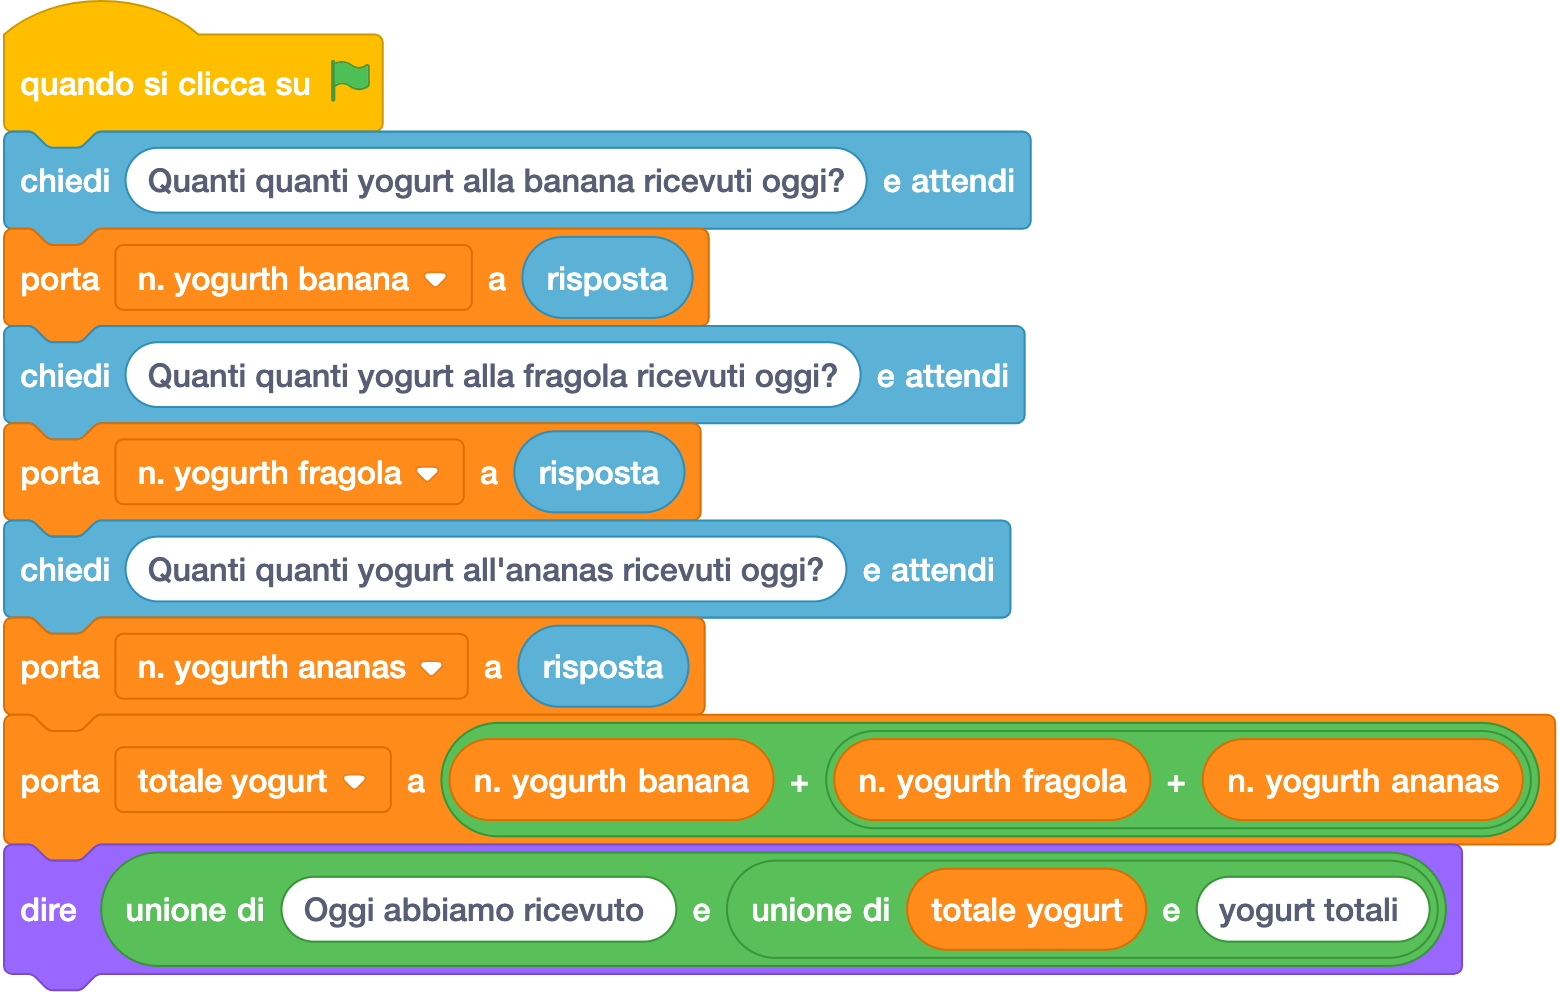
\includegraphics[width=0.8\linewidth]{img/cap2-scratch-programma.png}\label{credito:cap2-scratch-programma-1}
\end{center}

Ogni giorno, il responsabile potrà eseguire sul proprio computer questo programma senza più pensare a quale sia il procedimento: il computer eseguirà fedelmente le istruzioni al posto suo, gli chiederà in input i dati, e gli mostrerà il risultato.

Nella pratica scolastica può capitare di utilizzare il termine \textbf{algoritmi} per indicare solo le procedure che le alunne e gli alunni eseguono a volte meccanicamente (es. l'algoritmo per eseguire la divisione in colonna), cosa che può veicolare una visione procedurale della conoscenza lontana dalla comprensione concettuale e dal pensiero critico \parencite{crippa-etal-2025}. Questo è molto lontano dal senso informatico: infatti, gli informatici non hanno interesse a eseguire procedure sempre uguali e ripetitive--abbiamo inventato i computer proprio per eseguirle al posto nostro! Gli informatici sono molto più interessati a \textbf{inventare algoritmi} che risolvano problemi generali che si prestano poi ad essere automatizzati.


\subsection{Programmatore o esecutore?}


Se in generale gli informatici non amano essere ``esecutori'', per imparare l'informatica può essere utile, a volte, ``fare finta di essere un computer'', cioè eseguire alla lettera (secondo una precisa semantica) solo un insieme definito e limitato di istruzioni. Questo aiuta, quando si assumerà invece il ruolo di programmatori, a descrivere le elaborazioni che ci interessano in modo preciso e tenendo conto di ogni aspetto, senza lasciare nulla di implicito.

In alcune attività didattiche per l'introduzione dell'Informatica a scuola, però, viene posto l'accento solo sul ruolo di esecutore. È importante che le alunne e gli alunni riescano, a un certo punto, a costruire i propri programmi. Per questo motivo, nelle attività proposte in questa guida espliciteremo sempre quale ruolo (esecutore, programmatore o entrambi) assumono alunne e alunni, indicandoli con le seguenti icone.

\begin{center}
\ruoloProgrammatore\qquad\ruoloEsecutore
\end{center}

\begin{rimandiquaderno}
Anche nel volume studente vengono chiariti i ruoli di esecutore (ingranaggi) e programmatore (blocchetto verde), con due icone diverse.
\end{rimandiquaderno}

\section{Riferimenti}\label{riferimenti-1}

\printbibliography[heading=none,keyword={cap2},notcategory={attivita}]
